\documentclass[xcolor=dvipsnames
              ,handout
              ]{beamer} 

\usetheme{Madrid} 
%\setbeamertemplate{blocks}[shadow=false] 
\setbeamertemplate{navigation symbols}{} 
\setbeamertemplate{items}[square]
\setbeamertemplate{sections/subsections in toc}[square]

\definecolor{myblueend}{rgb}{0.058,0.132,0.42}
\definecolor{mybluemiddle}{rgb}{0.31,0.45,0.64}
\definecolor{mybluestart}{rgb}{0.17,0.28,0.48}
\definecolor{mygreen}{rgb}{0,0.7,0}
\definecolor{mylightgreen}{rgb}{0.7,1,0.7}
\definecolor{mylightblue}{rgb}{0.7,0.7,1}
\definecolor{mylightblack}{rgb}{0.7,0.7,0.7}
\definecolor{mylightred}{rgb}{1,0.7,0.7}
\definecolor{oproverblue}{RGB}{12,83,144}
\definecolor{oproveryellow}{RGB}{255,156,55}
\definecolor{mydarkgreen}{rgb}{0.17,0.48,0.28}
\definecolor{mydarkred}{rgb}{0.48,0.28,0.17}
\definecolor{grey}{rgb}{0.7,0.7,0.7}
\definecolor{darkgrey}{rgb}{0.5,0.5,0.5}

%\setbeamercolor{palette primary}{fg=white,bg=mybluestart}
%\setbeamercolor{palette secondary}{fg=white,bg=mybluestart}
%\setbeamercolor{palette tertiary}{fg=white,bg=mybluestart}
%\setbeamercolor{palette quaternary}{fg=white,bg=mybluestart}
\setbeamercolor{palette primary}{fg=white,bg=oproverblue}
\setbeamercolor{palette secondary}{fg=white,bg=oproverblue}
\setbeamercolor{palette tertiary}{fg=white,bg=oproverblue}
\setbeamercolor{palette quaternary}{fg=white,bg=oproverblue}
\setbeamercolor{titlelike}{parent=palette quaternary}

\setbeamercolor{item}{fg=oproverblue}
\setbeamercolor{block title}{fg=white,bg=oproverblue}
\setbeamercolor{block title example}{fg=white,bg=oproveryellow}
%\setbeamercolor{block title alert}{fg=white,bg=mydarkred}

\usefonttheme{serif}

%%
%% TOOLS
%% 
\newcommand{\opensmt}{{\sc OpenSMT}\xspace}
\newcommand{\yices}{{\sc Yices}\xspace}
\newcommand{\mathsat}{{\sc MathSAT}\xspace}
\newcommand{\cvcfour}{{\sc CVC4}\xspace}
\newcommand{\zthree}{{\sc Z3}\xspace}
\newcommand{\boolector}{{\sc Boolector}\xspace}
\newcommand{\verit}{{\sc veriT}\xspace}
\newcommand{\stp}{{\sc STP}\xspace}
\newcommand{\minisat}{{\sc MiniSAT}\xspace}
%%
%% BOOLEAN OPERATORS
%%
\newcommand{\swedge}{\,\wedge\,}
\newcommand{\svee}{\,\vee\,}
\newcommand{\impl}{\,\rightarrow\,}
%%
%% SMTLIB LOGICS
%% 
\newcommand{\Idl}{\ensuremath{\mathcal{IDL}}\xspace}
\newcommand{\Rdl}{\ensuremath{\mathcal{RDL}}\xspace}
\newcommand{\Uf}{\ensuremath{\mathcal{UF}}\xspace}
\newcommand{\Lia}{\ensuremath{\mathcal{LIA}}\xspace}
\newcommand{\Lra}{\ensuremath{\mathcal{LRA}}\xspace}
\newcommand{\Arrays}{\ensuremath{\mathcal{A}}\xspace}
\newcommand{\Bitvectors}{\ensuremath{\mathcal{BV}}\xspace}
\newcommand{\T}{\ensuremath{\mathcal{T}}\xspace}
\newcommand{\B}{\ensuremath{\mathcal{B}}\xspace}
%%
%% SETS
%%
\newcommand{\Int}{\ensuremath{\mathbb{Z}}\xspace}
\newcommand{\Rat}{\ensuremath{\mathbb{Q}}\xspace}
\newcommand{\Rea}{\ensuremath{\mathbb{R}}\xspace}
\newcommand{\Boo}{\ensuremath{\mathbb{B}}\xspace}
%%
%% SORTS
%%
\newcommand{\SInt}{{\tt Int}\xspace}
\newcommand{\SRea}{{\tt Real}\xspace}
\newcommand{\SBoo}{{\tt Bool}\xspace}
\newcommand{\SBv}[1]{{\tt BV}$_{[#1]}$\xspace}
%%
%% SMT specific
%%
\newcommand{\tconflict}{\T-conflict\xspace}
\newcommand{\tconflicts}{\T-conflicts\xspace}
\newcommand{\tterm}{\T-term\xspace}
\newcommand{\tterms}{\T-terms\xspace}
\newcommand{\tatom}{\T-atom\xspace}
\newcommand{\tatoms}{\T-atoms\xspace}
\newcommand{\tlit}{\T-literal\xspace}
\newcommand{\tlits}{\T-literals\xspace}
\newcommand{\tformula}{\T-formula\xspace}
\newcommand{\batom}{\B-atom\xspace}
\newcommand{\batoms}{\B-atoms\xspace}
\newcommand{\blit}{\B-literal\xspace}
\newcommand{\blits}{\B-literals\xspace}
\newcommand{\babst}[1]{#1^{\B}}
\newcommand{\tsolver}{\T-solver\xspace}
\newcommand{\tsolvers}{\T-solvers\xspace}
%%
%% SAT specific
%%
\newcommand{\dec}[2]{\stackrel{\textcolor{oproveryellow}{#2}}{#1}}
%%
%% BIT-VECTORS
%%
\newcommand{\w}[2]{\ensuremath{#1_{[#2]}}}
\newcommand{\band}{\,{\bf AND}\,}
\newcommand{\bor}{\,{\bf OR}\,}
\newcommand{\bnot}{{\bf NOT}\,}
\newcommand{\bitandsymb}{\,\, {\bf AND}}
\newcommand{\bit}[2]{#1\ensuremath{^#2}}
%%
%% IDL graphs
%%
\newcommand{\idlnode}[2]{\frac{#1}{#2}}
%%
%% LRA Solver
%%
\newcommand{\bas}{\ensuremath{\mathcal{B}}\xspace}
\newcommand{\nonbas}{\ensuremath{\mathcal{N}}\xspace}
%%
%% MISC
%%
\newcommand{\Lbrack}{\ensuremath{[\mspace{-3mu}[}}
\newcommand{\Rbrack}{\ensuremath{]\mspace{-3mu}]}}
\newcommand{\inter}[1]{\ensuremath{\Lbrack #1 \Rbrack}}
\newcommand{\COMMENT}[1]{}
\newcommand{\hl}[1]{\colorbox{oproveryellow}{\bf #1}}
\newcommand{\colfou}[1]{\textcolor{grey}{#1}}
\newcommand{\formulae}{formul\ae\xspace}
\newcommand{\smtsolvers}{SMT-solvers\xspace}
\newcommand{\smtsolver}{SMT-solver\xspace}
\newcommand{\satsolvers}{SAT-solvers\xspace}
\newcommand{\satsolver}{SAT-solver\xspace}
\newcommand{\bitvectors}{Bit-Vectors\xspace}
\newcommand{\bitvector}{Bit-Vector\xspace}
\newcommand{\colone}[1]{\textcolor{red}{#1}}
\newcommand{\coltwo}[1]{\textcolor{mygreen}{#1}}
\newcommand{\coloneat}[2]{\textcolor<#2>{red}{#1}}
\newcommand{\coltwoat}[2]{\textcolor<#2>{mygreen}{#1}}
\newcommand{\colfouat}[2]{\textcolor<#2>{grey}{#1}}
\newcommand{\claset}{\mathcal{C}}
\newcommand{\ra}[1]{\renewcommand{\arraystretch}{#1}}

\usepackage{epsfig}
\usepackage{graphicx}
\usepackage{color}
\usepackage{amstext}
\usepackage{amssymb}
\usepackage{amsfonts}
\usepackage{amsmath}
\usepackage{amsthm}
\usepackage{xspace}
\usepackage{multirow}
\usepackage{tabularx,colortbl}
\usepackage{alltt}
\usepackage{bussproofs}
\usepackage{algorithm2e}
\usepackage{datetime}
\usepackage{tikz}


\title[Summary and Exercises]{Satisfiability Modulo Theories\\ Lezione 10 - Summary of the course and exercises \\ {\tiny (slides revision: \today, \currenttime)}}
\author[R. Bruttomesso]{\large Roberto Bruttomesso}
\date{19 Ottobre 2012}
\institute[SMT]{\large Seminario di Logica Matematica \\(Corso Prof. Silvio Ghilardi)}
\logo{ \vspace{-6pt} \includegraphics[scale=0.15]{imgs/logo-ita.png} }

\begin{document}

\frame{\titlepage}

\begin{frame}
  \frametitle{Outline}
  \tableofcontents
\end{frame}

\section{Lecture 1 - Reduction to SAT}

\begin{frame}
  \frametitle{Solving SMT \formulae by reduction to SAT}

  \scriptsize

  Approaches to solve SMT \formulae are based on the observation
  that SMT can be {\bf reduced} to SAT, i.e., the purely Boolean
  Satisfiability Problem
  \vfill
  Consider for instance the \Lia formula
  $$
  \varphi\ \equiv\ (x - y \leq 0)\ \wedge\ (y - z \leq 0)\ \wedge\ ((z - x \leq -1)\ \vee\ (z - x \leq -2))
  $$
  We may use a Boolean variable $a$ to mean ``$x - y \leq 0$'' evaluates to $\top$
  in the model. Similarly we could use $b, c, d$ for the other \tatoms, obtaining
  $$
  \psi\ \equiv\ a \wedge b \wedge (c \vee d)
  $$
  \vfill
  \pause
  However we are not done with the encoding ! In fact altough $\mu^\Boo \equiv \{ a, b, c \}$ 
  is a (Boolean) model for $\psi$, the correspondent set of \tatoms $\{ x - y \leq 0, y - z \leq 0, z - x \leq -1 \}$
  is not consistent in \Lia: we cannot extend $\mu^\Boo$ to a model $\mu$ that satisfies $\varphi$.
  \pause
  \vfill
  This information can be added to the encoding in the following form
  $$ \neg( a \wedge b \wedge c )$$
  \pause
  \vfill
  Similarly we may derive {\bf all} the remaining incompatibilities
  $$ \neg( a \wedge b \wedge d )\quad\quad \neg( \neg a \wedge \neg b \wedge \neg c )\quad\quad \neg( \neg a \wedge \neg b \wedge \neg d )$$

\end{frame}

\begin{frame}
  \frametitle{Solving SMT \formulae by reduction to SAT}

  \scriptsize

  Initial \Lia formula
  $$
  \varphi \equiv (x - y \leq 0) \wedge (y - z \leq 0) \wedge ((z - x \leq -1) \vee (z - x \leq -2))
  $$
  Putting all the conditions together we get the Boolean formula
  $$ 
  \psi \equiv\ a \wedge b \wedge (c \vee d)\ \wedge\ \neg( a \wedge b \wedge c )\ \wedge\ \neg( a \wedge b \wedge d )\ \wedge\
  \neg( \neg a \wedge \neg b \wedge \neg c )\ \wedge\ \neg( \neg a \wedge \neg b \wedge \neg d )
  $$ \pause
  \vfill
  Starting from $\varphi$ we have
  \begin{enumerate}[$(i)$]
    \item encoded the structure of $\varphi$
    \item {\bf exhaustively} encoded all incompatible relations between \tatoms 
  \end{enumerate} 
  \vfill
  \begin{theorem}[Exercise 4 - correctness of the encoding]
    $\varphi$ is \T-satisfiable $\Leftrightarrow$ $\psi$ is satisfiable,
    where $\psi$ is obtained from $\varphi$ with the steps $(i)$-$(ii)$
  \end{theorem}

\end{frame}

\begin{frame}
  \frametitle{Exercise 4 - Proof}

  ($a_i$ is the Boolean variable corresponding to a \tatom $P_i$)
  \vfill

  ($\Rightarrow$)
  \medskip \\
  If $\varphi$ is \T-satisfiable, then it means that a model $\mu$ exists.
  A model $\mu^\Boo$ for $\psi$ can be defined with $\mu^\Boo(a_i) = \mu(P_i)$.
  \vfill\pause
  
  ($\Leftarrow$)
  \medskip \\
  Suppose that $\psi$ is satisfiable but $\varphi$ is not. If so, then
  there is a model $\mu^\Boo$ (e.g., $\{ \neg a_1, a_3 \}$) such that 
  its encoding (e.g., $(\neg P_1 \wedge P_3)$) represents an incompatible relation
  of \tatoms. But if it is an incompatible relation, than its negation was
  added to $\psi$ (e.g, $\neg ( a_1 \wedge a_3 )$), and it should not be satisfied
  by $\mu^\Boo$. Contradiction.
  
\end{frame}

\begin{frame}
  \frametitle{Exercize 2}

  \scriptsize

  Given the unsatisfiable formula 
  $$
  \psi \equiv\ a \wedge b \wedge (c \vee d)\ \wedge\ \neg( a \wedge b \wedge c )\ \wedge\ \neg( a \wedge b \wedge d )\ \wedge\
  \neg( \neg a \wedge \neg b \wedge \neg c )\ \wedge\ \neg( \neg a \wedge \neg b \wedge \neg d )
  $$
  show that $\neg( \neg a \wedge \neg b \wedge \neg c )$ and $\neg( \neg a \wedge \neg b \wedge \neg d )$ are redundant.
  \vfill\pause
  The last two clauses are redundant if 
  $$a \wedge b \wedge (c \vee d)\ \wedge\ \neg( a \wedge b \wedge c )\ \wedge\ \neg( a \wedge b \wedge d )$$
  is already unsatisfiable on its own. \pause In every model $a$ and $b$ must be assigned to $\top$. This simplifies
  the formula to
  $$(c \vee d)\ \wedge\ \neg( c )\ \wedge\ \neg( d )$$\pause
  Now in every model $c$ and $d$ must be assigned to $\bot$. This simplifies the formula to
  $$\bot$$

\end{frame}

\section{Lecture 3 - SAT-Solving}

\begin{frame}
  \frametitle{SAT-Solving}

  SAT-Solving is (the art of) finding the assignment satisfying all clauses
  \vfill
  The assignment evolves {\bf incrementally} by taking {\bf Decisions}, 
  starting from empty $\{\ \}$, but it can be {\bf backtracked} if found wrong
  \vfill
  The evolution of the assignment can be represented as a {\bf tree}
  \vfill
  \begin{tabular}{ccc}
    \begin{minipage}{.4\textwidth}
    $$
      \begin{array}{l}
      (\coltwoat{\neg a_1}{3-5} \vee a_3 \vee a_9) \\
      (\coloneat{\coltwoat{\neg a_2}{4}}{5} \vee \neg a_3 \vee a_4) \\
      (\coloneat{a_1}{3-5} \vee \coltwoat{\coloneat{a_2}{4}}{5}) \\
      (\neg a_4 \vee a_5 \vee a_{10})
      \end{array}
    $$
    \begin{overlayarea}{\textwidth}{.3cm}
      \only<1|handout:0>{$\{\ \}$}
      \only<2|handout:0>{$\{ \neg a_1 \}$}
      \only<3|handout:0>{$\{ \neg a_1, \neg a_2 \}$}
      \only<4|handout:0>{$\{ \neg a_1, a_2 \}$}
      \only<5>{$\{ \ldots \}$}
    \end{overlayarea}
    \end{minipage}
    & ~~~~ &
    \begin{minipage}{.4\textwidth}
    \begin{overlayarea}{\textwidth}{5cm}
      %\only<1|handout:0>{\scalebox{.7}{\input{sat_search_1.pdf_t}}}
      \only<1|handout:0>{\scalebox{.7}{\input{sat_search_1_1.pdf_t}}}
      \only<2|handout:0>{\scalebox{.7}{\input{sat_search_1_2.pdf_t}}}
      \only<3|handout:0>{\scalebox{.7}{\input{sat_search_1_3.pdf_t}}}
      \only<4|handout:0>{\scalebox{.7}{\input{sat_search_1_4.pdf_t}}}
      \only<5>{\scalebox{.7}{\input{sat_search_1_5.pdf_t}}}
    \end{overlayarea}
    \end{minipage}
  \end{tabular}

\end{frame}

\begin{frame}
  \frametitle{SAT-Solving}

  There are assignments which can be trivially driven towards the right direction.
  In the example below, given the current assignment, the third clause can be satisfied
  only by setting $a_2 \mapsto \top$ 
  \vfill
  \begin{tabular}{ccc}
    \begin{minipage}{.4\textwidth}
    $$
      \begin{array}{l}
      (\coltwoat{\neg a_1}{1-} \vee a_3 \vee a_9) \\
      (\coloneat{\neg a_2}{2-} \vee \neg a_3 \vee a_4) \\
      (\coloneat{a_1}{1-} \vee \coltwoat{a_2}{2-}) \\
      (\neg a_4 \vee a_5 \vee a_{10})
      \end{array}
    $$
    \begin{overlayarea}{\textwidth}{.3cm}
      \only<1|handout:0>{$\{ \neg a_1 \}$}
      \only<2->{$\{ \neg a_1, a_2 \}$}
    \end{overlayarea}
    \end{minipage}
    & ~~~~ &
    \begin{minipage}{.4\textwidth}
    \begin{overlayarea}{\textwidth}{4cm}
      \only<1|handout:0>{\scalebox{.7}{\input{sat_search_2_1.pdf_t}}}
      \only<2->{\scalebox{.7}{\input{sat_search_2_2.pdf_t}}}
    \end{overlayarea}
    \end{minipage}
  \end{tabular}
  \vfill
  \pause
  \pause
  This step is called {\bf Boolean Constraint Propagation} (BCP). It represents
  a {\bf forced} deduction. It triggers whenever all literals but one are assigned $\bot$
  $$
  (\colone{\neg a_1} \vee \colone{a_2} \vee \colone{\neg a_3} \vee \colone{a_4} \vee \neg a_5)
  $$

\end{frame}

\begin{frame}[fragile]
  \frametitle{SAT-Solving}

  {\bf Decision-level}: in an assignment, it is the number of decisions taken 
  \vfill
  Clearly, BCPs do not contribute to increase the decision level
  \vfill
  When necessary, we will indicate decision level on top of literals $\dec{a}{5}$ in the assignment 
  \vfill
  Example:
  \begin{center}
  \begin{tabular}{ccc}
    \begin{minipage}{.4\textwidth}
      \vfill
      $\{ \dec{a_{10}}{0}, \dec{\neg a_{1}}{1}, \dec{a_3}{2}, \dec{\neg a_4}{3}, \dec{a_5}{3} \}$
      \vfill
    \end{minipage}
    & &
    \begin{minipage}{.4\textwidth}
      \scalebox{.4}{\input{sat_search_4.pdf_t}}
    \end{minipage}
  \end{tabular}
  \end{center}
  
\end{frame}

\begin{frame}
  \frametitle{SAT-Solving}
  
  The process of finding the satisfying assignment is called {\bf search}, and
  in its basic version it evolves with {\bf Decisions}, {\bf BCPs}, and
  {\bf backtracking}

  \begin{center}
  \scalebox{.5}{\input{sat_search_3.pdf_t}}
  \end{center}

\end{frame}

\begin{frame}
  \frametitle{SAT-Solving}

  \scriptsize

  Consider the following scenario before and after BCP
  \vfill
  \begin{tabular}{ccc}
  \begin{minipage}{.4\textwidth}
  $$
  \begin{array}{l}
    \ldots \\
    (\colone{\neg a_{10}} \vee \colone{\neg a_1} \vee a_4) \\
    (\colone{a_3} \vee \colone{\neg a_1} \vee a_5) \\
    (\neg a_4 \vee a_6) \\
    (\neg a_5 \vee \neg a_6) \\
    \ldots \\
    \\
    \{ \dec{a_{10}}{0}, \dec{\neg a_3}{1}, \dec{a_7}{2}, \dec{\neg a_2}{3}, \dec{a_1}{4} \}
  \end{array}
  $$
  \end{minipage}
  & ~~~~ &
  \begin{minipage}{.5\textwidth}
  $$
  \begin{array}{l}
    \ldots \\
    (\colone{\neg a_{10}} \vee \colone{\neg a_1} \vee \coltwo{a_4}) \\
    (\colone{a_3} \vee \colone{\neg a_1} \vee \coltwo{a_5}) \\
    (\colone{\neg a_4} \vee \coltwo{a_6}) \\
    (\colone{\neg a_5} \vee \colone{\neg a_6}) \\
    \ldots \\
    \\
    \{ \dec{a_{10}}{0}, \dec{\neg a_3}{1}, \dec{a_7}{2}, \dec{\neg a_2}{3}, \dec{a_1}{4}, \dec{a_4}{4}, \dec{a_5}{4}, \dec{a_6}{4}\}
  \end{array}
  $$
  \end{minipage}
  \end{tabular}
  \vfill
  BCP leads to a conflict, but, what is the {\bf reason} for it ?
  Do $a_7$ and $a_2$ play any role ?
  \vfill
  Does it make sense to consider the assignments (which backtracking would produce) ?\\
  $\{ \dec{a_{10}}{0}, \dec{\neg a_3}{1}, \dec{\neg a_7}{2}, \dec{\neg a_2}{3}, \dec{a_1}{4} \}$ ---
  $\{ \dec{a_{10}}{0}, \dec{\neg a_3}{1}, \dec{a_7}{2}, \dec{\neg a_2}{3}, \dec{a_1}{4} \}$ ---
  $\{ \dec{a_{10}}{0}, \dec{\neg a_3}{1}, \dec{a_7}{2}, \dec{a_2}{3}, \dec{a_1}{4} \}$ \\
  \vfill
  No, because {\em whenever $a_{10}$, $\neg a_3$ is assigned, then $a_1$ must not be set to $\top$}.
  This translates to an additional clause, which can be {\em learnt}, i.e., it can be added to the formula 
  $$(\neg a_{10} \vee a_3 \vee \neg a_1)$$
   
\end{frame}

\begin{frame}
  \frametitle{SAT-Solving}

  \scriptsize

  In practice, we use {\bf resolution} steps to compute the learnt clause:
  \begin{itemize}
    \item we start from the clause with all literals to $\bot$ (conflicting clause)
    \item iteratively, we take the clause that propagated the last literal on the trail
	  and we apply resolution
    \item we stop when only one literal from the current decision level is left in the clause 
  \end{itemize}
  \vfill
  \begin{tabular}{ccc}
    \begin{minipage}{.4\textwidth}
      \scalebox{.4}{\input{ca_7.pdf_t}}
    \end{minipage}
    & ~~~~~~~~~~ &
    \begin{minipage}{.4\textwidth}
      \begin{tabular}{ccl}
	\hline
	Trail & dl & Reason \\
	\hline
	$a_{10}$   & 0 & $( a_{10} )$ \\
	$\neg a_3$ & 1 & Decision \\
	$a_7$      & 2 & Decision \\
	$\neg a_2$ & 3 & Decision \\
	$a_1$      & 4 & Decision \\
	$a_4$      & 4 & $(\neg a_{10} \vee \neg a_1 \vee a_4)$ \\
	$a_5$      & 4 & $(a_3 \vee \neg a_1 \vee a_5)$ \\
	$a_6$      & 4 & $(\neg a_4 \vee a_6)$ \\
	\hline
      \end{tabular}
      \medskip \\
      $\{ \dec{a_{10}}{0}, \dec{\neg a_3}{1}, \dec{a_7}{2}, \dec{\neg a_2}{3}, \dec{a_1}{4}, \dec{a_4}{4}, \dec{a_5}{4}, \dec{a_6}{4}\}$
    \end{minipage}
  \end{tabular}
  \vfill
  We say that $(\neg a_{10} \vee a_3 \vee \neg a_1)$ is the {\bf conflict clause} and it is the one we learn

\end{frame}

\begin{frame}
  \frametitle{Lecture 3 - Exercize 1}

  \scriptsize

  Consider the following clause set and assignment
  $$
  \begin{array}{l}
  (\neg a_1 \vee a_2) \\
  (\neg a_1 \vee a_3 \vee a_9) \\
  (\neg a_2 \vee \neg a_3 \vee a_4) \\
  (\neg a_4 \vee a_5 \vee a_{10}) \\
  (\neg a_4 \vee a_6 \vee a_{11}) \\
  (\neg a_5 \vee \neg a_6) \\
  (a_1 \vee a_7 \vee \neg a_{12}) \\
  (a_1 \vee a_8) \\
  (\neg a_7 \vee \neg a_8 \vee \neg a_{13}) \\
  \ldots \\ \\
  \{ \dec{\neg a_9}{1}, \dec{a_{12}}{2}, \dec{a_{13}}{2}, \dec{\neg a_{10}}{3}, \dec{\neg a_{11}}{3}, \ldots, \dec{a_1}{6}\}
  \end{array}
  $$
  \vfill
  \begin{itemize}
    \item Find the correct conflict clause
    \item Find the correct decision level to backtrack
  \end{itemize}

\end{frame}

\begin{frame}
  \frametitle{Lecture 3 - Exercize 1}

  \scriptsize

  \scalebox{.8}{
  \begin{tabular}{ccc}
    \begin{minipage}{.4\textwidth}
     $$
     \begin{array}{l}
     (\neg a_1 \vee a_2) \\
     (\neg a_1 \vee a_3 \vee a_9) \\
     (\neg a_2 \vee \neg a_3 \vee a_4) \\
     (\neg a_4 \vee a_5 \vee a_{10}) \\
     (\neg a_4 \vee a_6 \vee a_{11}) \\
     (\neg a_5 \vee \neg a_6) \\
     (a_1 \vee a_7 \vee \neg a_{12}) \\
     (a_1 \vee a_8) \\
     (\neg a_7 \vee \neg a_8 \vee \neg a_{13})
     \end{array}
     $$
    \end{minipage}
    & ~~~~~~ &
    \begin{minipage}{.4\textwidth}
      \begin{tabular}{ccl}
	\hline
	Trail & dl & Reason \\
	\hline
	$\neg a_{9}$  & 1 & Decision \\
	$a_{12}$      & 2 & Decision \\
	$a_{13}$      & 2 & (some clause) \\
	$\neg a_{10}$ & 3 & Decision \\
	$\neg a_{11}$ & 3 & (some clause) \\
	\ldots \\
	$a_1$         & 6 & Decision \\
	\hline 
	$a_2$         & 6 & $(\neg a_1 \vee a_2)$ \\
	$a_3$         & 6 & $(\neg a_1 \vee a_3 \vee a_9)$ \\
	$a_4$         & 6 & $(\neg a_2 \vee \neg a_3 \vee a_4)$ \\
	$a_5$         & 6 & $(\neg a_4 \vee a_5 \vee a_{10})$ \\
	$a_6$         & 6 & $(\neg a_4 \vee a_6 \vee a_{11})$ \\
	\hline
      \end{tabular}
      \bigskip \\
      $\{ \dec{\neg a_9}{1}, \dec{a_{12}}{2}, \dec{a_{13}}{2}, \dec{\neg a_{10}}{3}, \dec{\neg a_{11}}{3}, \ldots, \dec{a_1}{6} \}$
    \end{minipage}
  \end{tabular}}

  \vfill
  \pause

  \scalebox{.7}{
  \begin{minipage}{\textwidth}
    \begin{prooftree}
    \AxiomC{$(\neg a_5 \vee \neg a_6)$}
    \AxiomC{$(\neg a_4 \vee a_6 \vee a_{11})$}
    \BinaryInfC{$(\neg a_5 \vee \neg a_4 \vee a_{11})$}
    \AxiomC{$(\neg a_4 \vee a_5 \vee a_{10})$}
    \BinaryInfC{$(\neg a_4 \vee a_{10} \vee a_{11})$}
    \AxiomC{$(\neg a_2 \vee a_3 \vee a_4)$}
    \BinaryInfC{$(\neg a_2 \vee \neg a_3 \vee a_{10} \vee a_{11})$}
    \AxiomC{$(\neg a_2 \vee a_3 \vee a_9)$}
    \BinaryInfC{$(\neg a_2 \vee a_9 \vee a_{10} \vee a_{11})$}
    \AxiomC{$(\neg a_1 \vee a_2)$}
    \BinaryInfC{$(\neg a_1 \vee a_9 \vee a_{10} \vee a_{11})$}
    \end{prooftree}
  \end{minipage}
  }

  \vfill
  \pause
  Conflict clause: $(\neg a_1 \vee a_9 \vee a_{10} \vee a_{11})$ \pause \\
  Backtracking level: 3

\end{frame}

\section{Lecture 4 - The Lazy Approach}

\begin{frame}
  \frametitle{The Lazy Approach}

  \scriptsize

  Notice that
  \begin{itemize}
    \item Assignments $\mu$ of $\varphi$ are many (potentially $\infty$),
          infeasible to check if any of them is a model {\bf systematically}
    \item Models $\babst{\mu}$ of $\babst{\varphi}$ are finite in number,
          and easy to enumerate with a SAT-solver
    \item A model $\babst{\mu}$ is nothing but a {\bf conjunction of \tatoms},
          can be checked efficiently with a \tsolver
  \end{itemize}
  \vfill
  These observations suggest us a methodology
  to tackle the SMT(\T) problem
  \begin{itemize}
    \item Enumerate a Boolean model $\babst{\mu}$ of $\babst{\varphi}$ (abstraction). If no model 
	  exist we are done ($\varphi$ is unsatisfiable) 
    \item Check if $\babst{\mu}$ is satisfiable using the \tsolver. If so $\babst{\mu}$ can be extended 
          to a model $\mu$ of $\varphi$, and so we are done ! ($\varphi$ is satisfiable) 
    \item It not, we tell the SAT-solver not to enumerate $\babst{\mu}$ again,
          thus {\bf cutting away systematically an infinite number} 
	  of assignments for $\varphi$ (refinement) 
    \item It can be blocked by adding a clause $\neg \babst{\mu}$. Go up
    \item It terminates because there are finite Boolean models
  \end{itemize}

\end{frame}

\begin{frame}
  \frametitle{The Lazy Approach}

  \scriptsize
  
  The lazy approach falls into the so-called {\bf abstraction-refinement} 
  paradigm
  \vfill
  \begin{center}
  \scalebox{.5}{\subsection{Lazy Approach as Abstraction Refinement}

\begin{frame}
  \frametitle{Abstraction}
  Assigment relations
  \vfill
  \begin{center}
  \begin{tabular}{ccc}

    \begin{minipage}{.2\textwidth}

    $\babst{\varphi}$ \\
    \\
    \\
    \\
    \\
    \\
    $\varphi$ 

    \end{minipage}

    &

    \begin{minipage}{.55\textwidth}
      \begin{overlayarea}{\textwidth}{5cm}
	\only<1-3|handout:0>{\scalebox{.4}{\input{assignments_1.pdf_t}}}
	\only<4|handout:0>{\scalebox{.4}{\input{assignments_2.pdf_t}}}
	\only<5|handout:0>{\scalebox{.4}{\input{assignments_3.pdf_t}}}
	\only<6|handout:0>{\scalebox{.4}{\input{assignments_4.pdf_t}}}
	\only<7>{\scalebox{.4}{\input{assignments_5.pdf_t}}}
      \end{overlayarea}
    \end{minipage}

    &

    \begin{minipage}{.3\textwidth}

    \onslide<3->{$2^n$} \\
    \onslide<3->{($n = |\{ a_i \}|$)}\\
    \\
    \\
    \\
    \onslide<2->{$\infty$} \\ 
    \onslide<2->(can be) 

    \end{minipage}

  \end{tabular}
  \end{center}

\end{frame}

\begin{frame}
  \frametitle{Abstraction}
  Model relations
  \begin{itemize}
    \item<2-> if $\mu$ is a model for $\varphi$, then $\babst{\mu}$ is a model for $\babst{\varphi}$
    \item<3-> if $\babst{\mu}$ is not a model for $\babst{\varphi}$, then there is no $\mu$ that is a model for $\varphi$
    \item<4-> there may be some model $\babst{\mu}$ for $\babst{\varphi}$ that does not map to any model 
	      $\mu$ for $\varphi$
  \end{itemize}
  \vfill
  \begin{center}
  \begin{tabular}{cc}

    \begin{minipage}{.2\textwidth}

    $\babst{\varphi}$ \\
    \\
    \\
    \\
    \\
    \\
    $\varphi$ 

    \end{minipage}

    &

    \begin{minipage}{.7\textwidth}
      \begin{overlayarea}{\textwidth}{5cm}
	\only<1|handout:0>{\scalebox{.4}{\input{models_1.pdf_t}}}
	\only<2|handout:0>{\scalebox{.4}{\input{models_2.pdf_t}}}
	\only<3|handout:0>{\scalebox{.4}{\input{models_3.pdf_t}}}
	\only<4>{\scalebox{.4}{\input{models_4.pdf_t}}}
      \end{overlayarea}
    \end{minipage}

  \end{tabular}
  \end{center}

\end{frame}

\begin{frame}
  \frametitle{Abstraction Refinement}

  \scriptsize

  Notice that
  \begin{itemize}
    \item Assignments $\mu$ of $\varphi$ are many (potentially $\infty$),
          infeasible to check if any of them is a model {\bf systematically}
    \item Models $\babst{\mu}$ of $\babst{\varphi}$ are finite in number,
          and easy to enumerate with a SAT-solver
    \item A model $\babst{\mu}$ is nothing but a {\bf conjunction of \tatoms},
          can be checked efficiently with a \tsolver
  \end{itemize}
  \vfill
  \pause
  These observations suggest us a methodology
  to tackle the SMT(\T) problem
  \begin{itemize}
    \item Enumerate a Boolean model $\babst{\mu}$ of $\babst{\varphi}$ (abstraction). If no model 
	  exist we are done ($\varphi$ is unsatisfiable) \pause
    \item Check if $\babst{\mu}$ is satisfiable using the \tsolver. If so $\babst{\mu}$ can be extended 
          to a model $\mu$ of $\varphi$, and so we are done ! ($\varphi$ is satisfiable) \pause
    \item It not, we tell the SAT-solver not to enumerate $\babst{\mu}$ again,
          thus {\bf cutting away systematically an infinite number} 
	  of assignments for $\varphi$ (refinement) \pause
    \item It can be blocked by adding a clause $\neg \babst{\mu}$. Go up \pause
    \item It terminates because there are finite Boolean models
  \end{itemize}

\end{frame}

\begin{frame}
  \frametitle{Abstraction Refinement}

  \scriptsize
  
  The lazy approach falls into the so-called {\bf abstraction-refinement} 
  paradigm
  \vfill
  \begin{center}
  \scalebox{.5}{\subsection{Lazy Approach as Abstraction Refinement}

\begin{frame}
  \frametitle{Abstraction}
  Assigment relations
  \vfill
  \begin{center}
  \begin{tabular}{ccc}

    \begin{minipage}{.2\textwidth}

    $\babst{\varphi}$ \\
    \\
    \\
    \\
    \\
    \\
    $\varphi$ 

    \end{minipage}

    &

    \begin{minipage}{.55\textwidth}
      \begin{overlayarea}{\textwidth}{5cm}
	\only<1-3|handout:0>{\scalebox{.4}{\input{assignments_1.pdf_t}}}
	\only<4|handout:0>{\scalebox{.4}{\input{assignments_2.pdf_t}}}
	\only<5|handout:0>{\scalebox{.4}{\input{assignments_3.pdf_t}}}
	\only<6|handout:0>{\scalebox{.4}{\input{assignments_4.pdf_t}}}
	\only<7>{\scalebox{.4}{\input{assignments_5.pdf_t}}}
      \end{overlayarea}
    \end{minipage}

    &

    \begin{minipage}{.3\textwidth}

    \onslide<3->{$2^n$} \\
    \onslide<3->{($n = |\{ a_i \}|$)}\\
    \\
    \\
    \\
    \onslide<2->{$\infty$} \\ 
    \onslide<2->(can be) 

    \end{minipage}

  \end{tabular}
  \end{center}

\end{frame}

\begin{frame}
  \frametitle{Abstraction}
  Model relations
  \begin{itemize}
    \item<2-> if $\mu$ is a model for $\varphi$, then $\babst{\mu}$ is a model for $\babst{\varphi}$
    \item<3-> if $\babst{\mu}$ is not a model for $\babst{\varphi}$, then there is no $\mu$ that is a model for $\varphi$
    \item<4-> there may be some model $\babst{\mu}$ for $\babst{\varphi}$ that does not map to any model 
	      $\mu$ for $\varphi$
  \end{itemize}
  \vfill
  \begin{center}
  \begin{tabular}{cc}

    \begin{minipage}{.2\textwidth}

    $\babst{\varphi}$ \\
    \\
    \\
    \\
    \\
    \\
    $\varphi$ 

    \end{minipage}

    &

    \begin{minipage}{.7\textwidth}
      \begin{overlayarea}{\textwidth}{5cm}
	\only<1|handout:0>{\scalebox{.4}{\input{models_1.pdf_t}}}
	\only<2|handout:0>{\scalebox{.4}{\input{models_2.pdf_t}}}
	\only<3|handout:0>{\scalebox{.4}{\input{models_3.pdf_t}}}
	\only<4>{\scalebox{.4}{\input{models_4.pdf_t}}}
      \end{overlayarea}
    \end{minipage}

  \end{tabular}
  \end{center}

\end{frame}

\begin{frame}
  \frametitle{Abstraction Refinement}

  \scriptsize

  Notice that
  \begin{itemize}
    \item Assignments $\mu$ of $\varphi$ are many (potentially $\infty$),
          infeasible to check if any of them is a model {\bf systematically}
    \item Models $\babst{\mu}$ of $\babst{\varphi}$ are finite in number,
          and easy to enumerate with a SAT-solver
    \item A model $\babst{\mu}$ is nothing but a {\bf conjunction of \tatoms},
          can be checked efficiently with a \tsolver
  \end{itemize}
  \vfill
  \pause
  These observations suggest us a methodology
  to tackle the SMT(\T) problem
  \begin{itemize}
    \item Enumerate a Boolean model $\babst{\mu}$ of $\babst{\varphi}$ (abstraction). If no model 
	  exist we are done ($\varphi$ is unsatisfiable) \pause
    \item Check if $\babst{\mu}$ is satisfiable using the \tsolver. If so $\babst{\mu}$ can be extended 
          to a model $\mu$ of $\varphi$, and so we are done ! ($\varphi$ is satisfiable) \pause
    \item It not, we tell the SAT-solver not to enumerate $\babst{\mu}$ again,
          thus {\bf cutting away systematically an infinite number} 
	  of assignments for $\varphi$ (refinement) \pause
    \item It can be blocked by adding a clause $\neg \babst{\mu}$. Go up \pause
    \item It terminates because there are finite Boolean models
  \end{itemize}

\end{frame}

\begin{frame}
  \frametitle{Abstraction Refinement}

  \scriptsize
  
  The lazy approach falls into the so-called {\bf abstraction-refinement} 
  paradigm
  \vfill
  \begin{center}
  \scalebox{.5}{\input{ar.pdf_t}}
  \end{center}

\end{frame}
}
  \end{center}

\end{frame}
}
  \end{center}

\end{frame}

\begin{frame}
  \frametitle{The Lazy Approach}

  \scriptsize

  The interaction described naturally falls within the
  CDCL style, enriched with a \tsolver
      $$\varphi \equiv 
      (x=3 \vee \neg (x<3))\ \swedge\
      (x=3 \vee \neg (x>3))\ \swedge\
      (x>3 \vee \neg (x<3))\ \swedge\
      (x>3 \vee \neg (x=3))$$ 
  \vfill
  \begin{columns}

    \begin{column}{.5cm}
      \vspace{-165pt}
      $\babst{\varphi} \equiv$
    \end{column}

    \begin{column}{5cm}
      $(\coltwoat{\coloneat{a_1}{8-13}}{2-6} \vee \coltwoat{\neg a_2}{9-13})$ \\
      $(\coltwoat{\coloneat{a_1}{8-13}}{2-6} \vee \coltwoat{\coloneat{\neg a_3}{3-6}}{10-13})$ \\
      $(\coloneat{\coltwoat{a_3}{3-6}}{10-13} \vee \coltwoat{\neg a_2}{9-13})$ \\
      $(\coloneat{\coltwoat{a_3}{3-6}}{10-13} \vee \coloneat{\coltwoat{\neg a_1}{8-13}}{2-6})$ \\
      \onslide<6->{$(\coloneat{\coltwoat{\neg a_1}{10-13}}{6} \vee \coltwoat{\coloneat{\neg a_3}{6}}{10-13})$ \\}
      \onslide<7->{$(\coltwoat{\neg a_1}{8-13})$ \\}
      \onslide<13->{$(\coloneat{a_1}{13} \vee \coloneat{a_2}{13} \vee \coloneat{a_3}{13})$ \\}
      \onslide<14->{$(\ )$ \\}
      \bigskip
      $a_1 \equiv x=3$ \\
      $a_2 \equiv x<3$ \\
      $a_3 \equiv x>3$ \\
      \bigskip
      $\babst{\mu}$: $\{\ \only<2-6|handout:0>{a_1}\only<3-6|handout:0>{, a_3}\only<8-13|handout:0>{\neg a_1}\only<9-13|handout:0>{, \neg a_2}\only<10-13|handout:0>{, \neg a_3}\ \}$ \\
      \bigskip
      \begin{tabular}{rl}
      SAT-solver: & \only<1,4-5,11-12|handout:0>{Idle}\only<2|handout:0>{Decision}\only<3,8-10|handout:0>{BCP}\only<6,13|handout:0>{Learn}\only<7,14|handout:0>{Conf. Analysis, Backtrack}\only<15>{UNS} \\
        \tsolver: & \only<1,2,3,6-10,13->{Idle}\only<4,5,11,12|handout:0>{Is $\babst{\mu}$ \T-satisfiable ?}\only<5,12|handout:0>{ NO}
      \end{tabular}
    \end{column}

    \begin{column}{5cm}
      \begin{overlayarea}{5cm}{5cm}
	\only<1|handout:0>{\scalebox{.6}{\input{search_0.pdf_t}}}
	\only<2|handout:0>{\scalebox{.6}{\input{search_1.pdf_t}}}
	\only<3,4,5|handout:0>{\scalebox{.6}{\input{search_2.pdf_t}}}
	\only<6,7|handout:0>{\scalebox{.6}{\input{search_3.pdf_t}}}
	\only<8|handout:0>{\scalebox{.6}{\input{search_4.pdf_t}}}
	\only<9|handout:0>{\scalebox{.6}{\input{search_5.pdf_t}}}
	\only<10-12|handout:0>{\scalebox{.6}{\input{search_6.pdf_t}}}
	\only<13->{\scalebox{.6}{\input{search_7.pdf_t}}}
      \end{overlayarea}
    \end{column}

  \end{columns}

\end{frame}

\begin{frame}
  \frametitle{Lecture 4 - Exercize 1}

  \scriptsize

  \begin{tabular}{ccc}
    \begin{minipage}{.4\textwidth}
     $$
     \begin{array}{l}
     (a_1 \vee \neg a_2) \\
     (a_1 \vee \neg a_3) \\
     (a_3 \vee \neg a_2) \\
     (a_3 \vee \neg a_1) \\
     (\neg a_1 \vee \neg a_3)
     \end{array}
     $$
    \end{minipage}
    & ~~~~~~ &
    \begin{minipage}{.4\textwidth}
      \begin{tabular}{ccl}
	\hline
	Trail & dl & Reason \\
	\hline
	$a_1$ & 1 & Decision \\
	$a_3$ & 1 & $(a_3 \vee \neg a_1)$ \\
	\hline
      \end{tabular}
      \bigskip \\
      $\{ \dec{a_1}{1}, \dec{a_3}{1} \}$
    \end{minipage}
  \end{tabular}

  \vfill
  \pause

  \begin{minipage}{\textwidth}
    \begin{prooftree}
    \AxiomC{$(\neg a_1 \vee \neg a_3)$}
    \AxiomC{$( a_3 \vee \neg a_1 )$}
    \BinaryInfC{$(\neg a_1)$}
    \end{prooftree}
  \end{minipage}

  \vfill
  \pause
  Conflict clause: $(\neg a_1)$ \pause \\
  Backtracking level: 0
\end{frame}

\begin{frame}
  \frametitle{Lecture 4 - Exercize 1}

  \scriptsize

  \begin{tabular}{ccc}
    \begin{minipage}{.4\textwidth}
     $$
     \begin{array}{l}
     (a_1 \vee \neg a_2) \\
     (a_1 \vee \neg a_3) \\
     (a_3 \vee \neg a_2) \\
     (a_3 \vee \neg a_1) \\
     (\neg a_1 \vee \neg a_3) \\
     (\neg a_1) \\
     (a_1 \vee a_2 \vee a_3)
     \end{array}
     $$
    \end{minipage}
    & ~~~~~~ &
    \begin{minipage}{.4\textwidth}
      \begin{tabular}{ccl}
	\hline
	Trail & dl & Reason \\
	\hline
	$\neg a_1$ & 0 & $(\neg a_1)$ \\
	$\neg a_2$ & 0 & $(a_1 \vee \neg a_2)$ \\
	$\neg a_3$ & 0 & $(a_1 \vee \neg a_3)$ \\
	\hline
      \end{tabular}
      \bigskip \\
      $\{ \neg \dec{a_1}{0}, \neg \dec{a_2}{0}, \neg \dec{a_3}{0} \}$
    \end{minipage}
  \end{tabular}

  \vfill
  \pause

  \begin{minipage}{\textwidth}
    \begin{prooftree}
    \AxiomC{$(a_1 \vee a_2 \vee a_3)$}
    \AxiomC{$(a_3 \vee \neg a_1)$}
    \BinaryInfC{$(a_1 \vee a_2)$}
    \AxiomC{$(a_1 \vee \neg a_2)$}
    \BinaryInfC{$(a_1)$}
    \AxiomC{$(\neg a_1)$}
    \BinaryInfC{$\bot$}
    \end{prooftree}
  \end{minipage}

  \vfill
  \pause
  Conflict clause: $\bot$ \pause \\
  Backtracking level: 0
\end{frame}

\section{Lecture 5 - A \tsolver for \Idl}

\begin{frame}
  \frametitle{A \tsolver for \Idl}

  \scriptsize

  The constraint $\quad x - y \leq c \quad$ says that 
  
  \begin{center}
    ``the distance between $x$ and $y$ is at most $c$''
  \end{center}

  This can be encoded as $(x,y;c)$

  \begin{center}
    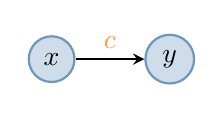
\begin{tikzpicture}[auto]

%
% Styles
%
\tikzstyle{vertex} = [circle,draw=oproverblue!60,fill=oproverblue!20,thick]
\tikzstyle{edge}   = [->,>=stealth,thick]
\tikzstyle{weight} = [color=oproveryellow]

\node[vertex] (x) at (2,0)   {$x$};
\node[vertex] (y) at (3.5,0) {$y$};

\draw[edge] (x) -- node[weight] {$c$} (y);

\end{tikzpicture}

  \end{center}

  \vfill
  So, a set $\babst{\mu}$ can be encoded as a graph. Concrete example:

  \begin{columns}

    \begin{column}{.3\textwidth}
      \ra{1.3}
      $$
      \begin{array}{rcr}
	x - y & \leq & 8   \\
	y - z & \leq & -1  \\
	z - x & \leq & -6  \\
	z - w & \leq & 2   \\
	w - x & \leq & -10 \\
	w - t & \leq & 0   \\
	t - x & \leq & 3     
      \end{array}
      $$
    \end{column}

    \begin{column}{.6\textwidth}
      \begin{center}
	\begin{frame}
  \frametitle{An Example}

  \scriptsize

  Consider the following problem

  \begin{overlayarea}{\textwidth}{1cm}
    \only<1|handout:0>{$$ x_1 - x_2 \leq 8\ \swedge\ x_2 - x_3 \leq -1\ \swedge\ x_3 - x_4 \leq 2\ \swedge\ x_4 - x_1 \leq -10 $$} 
    \only<2->{$$ x_5 \leq 8\ \swedge\ x_6 \leq -1\ \swedge\ x_7 \leq 2\ \swedge\ x_8 \leq -10 $$} 
  \end{overlayarea}

  \onslide<2->{
  \begin{columns}

  \begin{column}{.4\textwidth}
  \begin{center}
  Tableau
  \end{center}
  $$
  \only<2-4|handout:0>{
  \begin{array}{rcl}
    x_5 & = & x_1 - x_2  \\ 
    x_6 & = & x_2 - x_3  \\ 
    x_7 & = & x_3 - x_4  \\ 
    x_8 & = & x_4 - x_1  \\ 
  \end{array}}
  \only<5-7|handout:0>{
  \begin{array}{rcl}
    x_5 & = & x_1 - x_2  \\ 
    x_3 & = & x_2 - x_6  \\ 
    x_7 & = & x_2 - x_6 - x_4  \\ 
    x_8 & = & x_4 - x_1  \\ 
  \end{array}}
  \only<8|handout:0>{
  \begin{array}{rcl}
    x_5 & = & x_4 - x_8 - x_2  \\ 
    x_3 & = & x_2 - x_6  \\ 
    x_7 & = & x_2 - x_6 - x_4  \\ 
    x_1 & = & x_4 - x_8  \\ 
  \end{array}}
  \only<9,10>{
  \begin{array}{rcl}
    x_2 & = & x_4 - x_8 - x_5  \\ 
    x_3 & = & x_4 - x_8 - x_5 - x_6  \\ 
    \coloneat{x_7}{10} & \coloneat{=}{10} & \coloneat{- x_5 -x_8 - x_6}{10} \\ 
    x_1 & = & x_4 - x_8  \\ 
  \end{array}}
  $$
  \end{column}

  \begin{column}{.3\textwidth}
  \begin{center}
  $lb$~~~~~~~Bounds~~~~~~~$ub$
  \end{center}
  $$
  \begin{array}{rcccl}
    - \infty & \leq & x_5 & \leq & \only<2|handout:0>{\infty}\only<3->{8} \\
    - \infty & \leq & x_6 & \leq & \only<2,3|handout:0>{\infty}\only<4->{-1} \\
    - \infty & \leq & x_7 & \leq & \only<2-5|handout:0>{\infty}\only<6->{2} \\
    - \infty & \leq & x_8 & \leq & \only<2-6|handout:0>{\infty}\only<7->{-10} \\
  \end{array}
  $$
  \end{column}

  \begin{column}{.3\textwidth}
  \begin{center}
  $\mu$
  \end{center}
  $$
  \begin{array}{rcl}
  x_1 & \mapsto & \only<2-7|handout:0>{0}\only<8->{10} \\
  x_2 & \mapsto & \only<2-8|handout:0>{0}\only<9->{2} \\
  x_3 & \mapsto & \only<2-4|handout:0>{0}\only<5->{1} \\
  x_4 & \mapsto & 0 \\ 
  x_5 & \mapsto & \only<2-7|handout:0>{0}\only<8|handout:0>{10}\only<9->{8} \\
  x_6 & \mapsto & \only<2-4|handout:0>{0}\only<5->{-1} \\
  x_7 & \mapsto & \only<2-4|handout:0>{0}\only<5-8|handout:0>{1}\only<9->{3} \\
  x_8 & \mapsto & \only<2-7|handout:0>{0}\only<8->{-10} 
  \end{array}
  $$
  \end{column}

  \end{columns}
  }
  \vfill
  \begin{overlayarea}{\textwidth}{1cm}
    \only<3|handout:0>{Receiving $x_5 \leq 8$: OK}
    \only<4|handout:0>{Receiving $x_6 \leq -1$: $\mu(x_6)$ out of bounds}
    \only<5|handout:0>{$Pivot(x_6,x_3)$, $Update(x_6,-1)$. Values of $x_3$ and $x_7$ change as well}
    \only<6|handout:0>{Receiving $x_7 \leq 2$: OK}
    \only<7|handout:0>{Receiving $x_8 \leq -10$: $\mu(x_8)$ out of bounds}
    \only<8|handout:0>{$Pivot(x_8,x_1)$, $Update(x_8,-10)$. Values of $x_5$ and $x_1$ change as well. $\mu(x_5)$ out of bounds}
    \only<9|handout:0>{$Pivot(x_5,x_2)$, $Update(x_5,8)$. Values of $x_2$ and $x_7$ change as well. $\mu(x_7)$ out of bounds}
    \only<10>{Cannot find suitable variable for pivoting ($ChoosePivot(x_7)$ == $undef$). Return $unsat$}
  \end{overlayarea}

\end{frame}

      \end{center}
    \end{column}

  \end{columns}
  \vfill
  $G( V, E )$: $V = \{ x, y, z, w, t \}$, $E = \{ (x,y;8), (y,z;-1), (z,x;-6), (z,w;2), (w,x;-10), \ldots \}$ 

\end{frame}

\begin{frame}
  \frametitle{A \tsolver for \Idl}

  \scriptsize

    \begin{theorem}[Translation]
      \label{the:idl}
      $\babst{\mu}$ is \Idl-unsatisfiable 
      \begin{center}
      iff
      \end{center}
      there is a {\bf negative cycle} in the corresponging graph $G(V,E)$
    \end{theorem}

  \vfill
  E.g.:

  \begin{columns}

    \begin{column}{.3\textwidth}
      \ra{1.3}
      $$
      \begin{array}{rcr}
	\coloneat{x - y}{1} & \coloneat{\leq}{1} & \coloneat{8}{1}   \\
	\coloneat{y - z}{1} & \coloneat{\leq}{1} & \coloneat{-1}{1}  \\
	\colfouat{z - x}{1} & \colfouat{\leq}{1} & \colfouat{-6}{1}  \\
	\coloneat{z - w}{1} & \coloneat{\leq}{1} & \coloneat{2}{1}   \\
	\coloneat{w - x}{1} & \coloneat{\leq}{1} & \coloneat{-10}{1} \\
	\colfouat{w - t}{1} & \colfouat{\leq}{1} & \colfouat{0}{1}   \\
	\colfouat{t - x}{1} & \colfouat{\leq}{1} & \colfouat{3}{1}     
      \end{array}
      $$
    \end{column}

    \begin{column}{.6\textwidth}
      \begin{center}
	\begin{overlayarea}{.5\textwidth}{3cm}
	  %\only<2|handout:0>{\begin{frame}
  \frametitle{An Example}

  \scriptsize

  Consider the following problem

  \begin{overlayarea}{\textwidth}{1cm}
    \only<1|handout:0>{$$ x_1 - x_2 \leq 8\ \swedge\ x_2 - x_3 \leq -1\ \swedge\ x_3 - x_4 \leq 2\ \swedge\ x_4 - x_1 \leq -10 $$} 
    \only<2->{$$ x_5 \leq 8\ \swedge\ x_6 \leq -1\ \swedge\ x_7 \leq 2\ \swedge\ x_8 \leq -10 $$} 
  \end{overlayarea}

  \onslide<2->{
  \begin{columns}

  \begin{column}{.4\textwidth}
  \begin{center}
  Tableau
  \end{center}
  $$
  \only<2-4|handout:0>{
  \begin{array}{rcl}
    x_5 & = & x_1 - x_2  \\ 
    x_6 & = & x_2 - x_3  \\ 
    x_7 & = & x_3 - x_4  \\ 
    x_8 & = & x_4 - x_1  \\ 
  \end{array}}
  \only<5-7|handout:0>{
  \begin{array}{rcl}
    x_5 & = & x_1 - x_2  \\ 
    x_3 & = & x_2 - x_6  \\ 
    x_7 & = & x_2 - x_6 - x_4  \\ 
    x_8 & = & x_4 - x_1  \\ 
  \end{array}}
  \only<8|handout:0>{
  \begin{array}{rcl}
    x_5 & = & x_4 - x_8 - x_2  \\ 
    x_3 & = & x_2 - x_6  \\ 
    x_7 & = & x_2 - x_6 - x_4  \\ 
    x_1 & = & x_4 - x_8  \\ 
  \end{array}}
  \only<9,10>{
  \begin{array}{rcl}
    x_2 & = & x_4 - x_8 - x_5  \\ 
    x_3 & = & x_4 - x_8 - x_5 - x_6  \\ 
    \coloneat{x_7}{10} & \coloneat{=}{10} & \coloneat{- x_5 -x_8 - x_6}{10} \\ 
    x_1 & = & x_4 - x_8  \\ 
  \end{array}}
  $$
  \end{column}

  \begin{column}{.3\textwidth}
  \begin{center}
  $lb$~~~~~~~Bounds~~~~~~~$ub$
  \end{center}
  $$
  \begin{array}{rcccl}
    - \infty & \leq & x_5 & \leq & \only<2|handout:0>{\infty}\only<3->{8} \\
    - \infty & \leq & x_6 & \leq & \only<2,3|handout:0>{\infty}\only<4->{-1} \\
    - \infty & \leq & x_7 & \leq & \only<2-5|handout:0>{\infty}\only<6->{2} \\
    - \infty & \leq & x_8 & \leq & \only<2-6|handout:0>{\infty}\only<7->{-10} \\
  \end{array}
  $$
  \end{column}

  \begin{column}{.3\textwidth}
  \begin{center}
  $\mu$
  \end{center}
  $$
  \begin{array}{rcl}
  x_1 & \mapsto & \only<2-7|handout:0>{0}\only<8->{10} \\
  x_2 & \mapsto & \only<2-8|handout:0>{0}\only<9->{2} \\
  x_3 & \mapsto & \only<2-4|handout:0>{0}\only<5->{1} \\
  x_4 & \mapsto & 0 \\ 
  x_5 & \mapsto & \only<2-7|handout:0>{0}\only<8|handout:0>{10}\only<9->{8} \\
  x_6 & \mapsto & \only<2-4|handout:0>{0}\only<5->{-1} \\
  x_7 & \mapsto & \only<2-4|handout:0>{0}\only<5-8|handout:0>{1}\only<9->{3} \\
  x_8 & \mapsto & \only<2-7|handout:0>{0}\only<8->{-10} 
  \end{array}
  $$
  \end{column}

  \end{columns}
  }
  \vfill
  \begin{overlayarea}{\textwidth}{1cm}
    \only<3|handout:0>{Receiving $x_5 \leq 8$: OK}
    \only<4|handout:0>{Receiving $x_6 \leq -1$: $\mu(x_6)$ out of bounds}
    \only<5|handout:0>{$Pivot(x_6,x_3)$, $Update(x_6,-1)$. Values of $x_3$ and $x_7$ change as well}
    \only<6|handout:0>{Receiving $x_7 \leq 2$: OK}
    \only<7|handout:0>{Receiving $x_8 \leq -10$: $\mu(x_8)$ out of bounds}
    \only<8|handout:0>{$Pivot(x_8,x_1)$, $Update(x_8,-10)$. Values of $x_5$ and $x_1$ change as well. $\mu(x_5)$ out of bounds}
    \only<9|handout:0>{$Pivot(x_5,x_2)$, $Update(x_5,8)$. Values of $x_2$ and $x_7$ change as well. $\mu(x_7)$ out of bounds}
    \only<10>{Cannot find suitable variable for pivoting ($ChoosePivot(x_7)$ == $undef$). Return $unsat$}
  \end{overlayarea}

\end{frame}
}
	  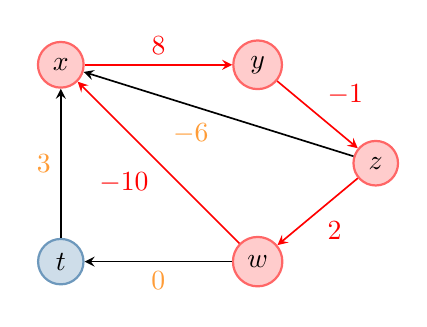
\begin{tikzpicture}[auto]

%
% Styles
%
\tikzstyle{vertex}   = [circle,draw=oproverblue!60,fill=oproverblue!20,thick]
\tikzstyle{edge}     = [->,>=stealth,semithick]
\tikzstyle{weight}   = [color=oproveryellow]
\tikzstyle{hlvertex} = [circle,draw=red!60,fill=red!20,thick]
\tikzstyle{hledge}   = [->,>=stealth,semithick,draw=red]
\tikzstyle{hlweight} = [color=red]

\node[hlvertex] (x) at (  1, 0)    {$x$};
\node[hlvertex] (y) at (3.5, 0)    {$y$};
\node[hlvertex] (z) at (  5,-1.25) {$z$};
\node[hlvertex] (w) at (3.5,-2.5)  {$w$};
\node[vertex] (t) at (  1,-2.5)  {$t$};

\draw[hledge] (x) -- node[hlweight] {$8$}   (y);
\draw[hledge] (y) -- node[hlweight] {$-1$}  (z);
\draw[edge]   (z) -- node[weight] {$-6$}  (x);
\draw[hledge] (z) -- node[hlweight] {$2$}   (w);
\draw[hledge] (w) -- node[hlweight] {$-10$} (x);
\draw[edge]   (w) -- node[weight] {$0$}   (t);
\draw[edge]   (t) -- node[weight] {$3$}   (x);

\end{tikzpicture}

	\end{overlayarea}
      \end{center}
    \end{column}

  \end{columns}

\end{frame}

\begin{frame}
  \frametitle{Lecture 5 - Exercize 4}
  
  \scriptsize

  Let's first recall the notion of {\bf minimality}
  \begin{center}
  A conflict $\nu^\Boo$ is {\bf minimal} if it does not contain redundant \tatoms
  \end{center}
  A \tatom $P$ in a conflict $\nu^\Boo$ is redundant if $\nu^\Boo \setminus \{ P \}$
  is still a conflict
  \vfill
  So, how do we check, in general, that a conflict $\nu^\Boo = \{ P_1, \ldots, P_n \}$ is minimal ?
  Iteratively for $i=1,\ldots,n$, we see if $\nu^\Boo \setminus \{ P_i \}$ is still a conflict.
  \vfill\pause
  In the case of difference logic every conflict is minimal {\bf by construction}. In fact $\nu^\Boo$ 
  is a conflict if and only if it is a {\bf cycle} with negative sum.
  \vfill
  Doing $\nu^\Boo \setminus \{ P_i \}$ is equivalent to breaking the cycle, no matter what $P_i$.
  Therefore all \tatoms are not redundant, and so conflicts are minimal.

\end{frame}

\begin{frame}
  \frametitle{Lecture 5 - Exercize 5}

  \scriptsize

  Prove
  \vfill

  \begin{exampleblock}{Observation 2}
    A set of constraints \\
    $\{\ \colone{x_1} - x_2 \leq c_1,\ x_2 - x_3 \leq c_2,\ \ldots,\ x_{n-1} - \coltwo{x_n} \leq c_{n-1}\ \}$ \\
    implies 
    $\quad\quad\colone{x_1} - \coltwo{x_n} \leq c_n\quad\quad$ 
    iff 
    $\quad\quad c_1 + c_2 + \ldots c_{n-1} \leq c_n$
  \end{exampleblock}

  \vfill
  using
  \vfill

  \begin{lemma}[Farka's Lemma for \Idl]
    $\babst{\mu}$ is unsatisfiable iff there exists a subset 
    $\babst{\nu} = \{\ \coltwo{x_1} - x_2 \leq c_1,\ x_2 - x_3 \leq c_2,\ \ldots,\ x_n - \coltwo{x_1} \leq c_n\ \}$ of $\babst{\mu}$
    such that $c_1 + \ldots + c_n < 0$
  \end{lemma}

\end{frame}

\begin{frame}
  \frametitle{Lecture 5 - Exercize 5}

  \scriptsize

  \begin{exampleblock}{Observation 2}
    A set of constraints \\
    $\{\ \colone{x_1} - x_2 \leq c_1,\ x_2 - x_3 \leq c_2,\ \ldots,\ x_{n-1} - \coltwo{x_n} \leq c_{n-1}\ \}$ \\
    implies 
    $\quad\quad\colone{x_1} - \coltwo{x_n} \leq c_n\quad\quad$ 
    iff 
    $\quad\quad c_1 + c_2 + \ldots c_{n-1} \leq c_n$
  \end{exampleblock}

  \vfill
  is better formalized as
  \vfill

  \begin{center}
  $(\colone{x_1} - x_2 \leq c_1\ \wedge\ x_2 - x_3 \leq c_2\ \wedge\ \ldots\ \wedge\ x_{n-1} - \coltwo{x_n} \leq c_{n-1}) \rightarrow (\colone{x_1} - \coltwo{x_n} \leq d_n)$ \\
  is valid iff \\
  $c_1 + c_2 + \ldots c_{n-1} \leq d_n$
  \end{center}

  \begin{lemma}[Farka's Lemma for \Idl]
    $\babst{\mu}$ is unsatisfiable iff there exists a subset 
    $\babst{\nu} = \{\ \coltwo{x_1} - x_2 \leq c_1,\ x_2 - x_3 \leq c_2,\ \ldots,\ x_n - \coltwo{x_1} \leq c_n\ \}$ of $\babst{\mu}$
    such that $c_1 + \ldots + c_n < 0$
  \end{lemma}

  \vfill
  is better formalized as
  \vfill

  \begin{center}
  $\colone{x_1} - x_2 \leq c_1\ \wedge\ x_2 - x_3 \leq c_2\ \wedge\ \ldots\ \wedge\ x_{n-1} - x_n \leq c_{n-1}\ \wedge\ x_n - \colone{x_1} \leq c_n$ \\
  is unsatisfiable iff \\
  $c_1 + c_2 + \ldots c_{n-1} + c_n < 0$
  \end{center}

\end{frame}

\begin{frame}
  \frametitle{Lecture 5 - Exercize 5}

  \scriptsize

  \begin{center}
  $(\colone{x_1} - x_2 \leq c_1\ \wedge\ x_2 - x_3 \leq c_2\ \wedge\ \ldots\ \wedge\ x_{n-1} - \coltwo{x_n} \leq c_{n-1}) \rightarrow (\colone{x_1} - \coltwo{x_n} \leq d_n)$ \\
  is valid iff \\
  $c_1 + c_2 + \ldots c_{n-1} \leq d_n$
  \end{center}

  \vfill
  is equivalent to (using the well-known fact: $\varphi \rightarrow \psi$ is valid iff $\varphi \wedge \neg \psi$ is unsat)
  \vfill

  \begin{center}
  $\colone{x_1} - x_2 \leq c_1\ \wedge\ x_2 - x_3 \leq c_2\ \wedge\ \ldots\ \wedge\ x_{n-1} - \coltwo{x_n} \leq c_{n-1}\ \wedge\ \neg(\colone{x_1} - \coltwo{x_n} \leq d_n)$ \\
  is unsatisfiable iff \\
  $c_1 + c_2 + \ldots c_{n-1} \leq d_n$
  \end{center}

  \vfill\pause
  which is equivalent to (using the fact $\neg (x - y \leq c)\ \Longleftrightarrow\ y - x \leq - c - 1$)
  \vfill

  \begin{center}
  $\colone{x_1} - x_2 \leq c_1\ \wedge\ x_2 - x_3 \leq c_2\ \wedge\ \ldots\ \wedge\ x_{n-1} - \coltwo{x_n} \leq c_{n-1}\ \wedge\ \coltwo{x_n} - \colone{x_1} \leq - d_n - 1$ \\
  is unsatisfiable iff \\
  $c_1 + c_2 + \ldots c_{n-1} \leq d_n$
  \end{center}

  \vfill\pause
  which is equivalent to (using the fact $c \leq d\ \Longleftrightarrow\ c - d \leq 0\ \Longleftrightarrow\ c - d - 1 < 0$)
  \vfill

  \begin{center}
  $\colone{x_1} - x_2 \leq c_1\ \wedge\ x_2 - x_3 \leq c_2\ \wedge\ \ldots\ \wedge\ x_{n-1} - x_n \leq c_{n-1} \wedge x_n - \colone{x_1} \leq - d_n - 1$ \\
  is unsatisfiable iff \\
  $c_1 + c_2 + \ldots c_{n-1} - d_n - 1 < 0$
  \end{center}

  \vfill
  which is Farka's Lemma if we set $c_n \equiv - d_n - 1$

\end{frame}

\section{Lecture 6 - A \tsolver for \Lra}

\begin{frame}
  \frametitle{A \tsolver for \Lra}

  \scriptsize

  \begin{columns}

  \begin{column}{.4\textwidth}
  \begin{center}
  Tableau
  \end{center}
  $$
  \begin{array}{rcl}
    & \ldots \\                             
    x_1 & = & 3 x_2 - 4 x_3 + 2 x_4 - x_5 \\ 
    & \ldots \\                             
    \\
    \\
  \end{array}
  $$
  \end{column}

  \begin{column}{.3\textwidth}
  \begin{center}
  $lb$~~~~~~~Bounds~~~~~~~$ub$
  \end{center}
  $$
  \begin{array}{rcccl}
     -4 & \leq & x_1 & \leq & 10 \\
      1 & \leq & x_2 & \leq & 3 \\
     -4 & \leq & x_3 & \leq & -1 \\
      1 & \leq & x_4 & \leq & 2 \\
     -1 & \leq & x_5 & \leq & 10 \\
  \end{array}
  $$
  \end{column}

  \begin{column}{.3\textwidth}
  \begin{center}
  $\mu$
  \end{center}
  $$
  \begin{array}{rcl}
  x_1 & \mapsto & \colone{12} \\
  x_2 & \mapsto & 1 \\
  x_3 & \mapsto & -1 \\
  x_4 & \mapsto & 2 \\
  x_5 & \mapsto & -1 
  \end{array}
  $$
  \end{column}

  \end{columns}
  \vfill
  which among $\nonbas = \{ x_2, x_3, x_4 \}$ do I choose for pivoting ? Clearly, the value of $\mu(x_1)$
  is too high, I have to decrease it by playing with the values of \nonbas: 
  \begin{itemize}
    \item $  3 x_2$ cannot decrease, as $\mu(x_2) = lb(x_2)$ and cannot be moved down
    \item $- 4 x_3$ cannot decrease, as $\mu(x_3) = ub(x_3)$ and cannot be moved up
    \item $  2 x_4$ can decrease, as  $\mu(x_4) = ub(x_4)$, and can be moved down
    \item $-   x_5$ can decrease, as  $\mu(x_5) = lb(x_5)$, and can be moved up
  \end{itemize}
  \vfill
  both $x_4$ and $x_5$ are therefore good candidates for pivoting. To avoid loops, 
  choose variable with smallest subscript (Bland's Rule). This rule is not necessarily
  efficient, though

\end{frame}

\begin{frame}
  \frametitle{A \tsolver for \Lra}

  \scriptsize

  There might be cases in which {\bf no suitable variable for pivoting can be found}.
  This indicates unsatisfiability. Consider the following where we have just asserted $x_1 \leq 9$
  \vfill
  \begin{columns}

  \begin{column}{.4\textwidth}
  \begin{center}
  Tableau
  \end{center}
  $$
  \begin{array}{rcl}
    & \ldots \\                             
    x_1 & = & 3 x_2 - 4 x_3 + 2 x_4 - x_5 \\ 
    & \ldots \\                             
    \\
    \\
  \end{array}
  $$
  \end{column}

  \begin{column}{.3\textwidth}
  \begin{center}
  $lb$~~~~~~~Bounds~~~~~~~$ub$
  \end{center}
  $$
  \begin{array}{rcccl}
     -4 & \leq & x_1 & \leq & 9 \\
      1 & \leq & x_2 & \leq & 3 \\
     -4 & \leq & x_3 & \leq & -1 \\
      2 & \leq & x_4 & \leq & 2 \\
     -1 & \leq & x_5 & \leq & -1 \\
  \end{array}
  $$
  \end{column}

  \begin{column}{.3\textwidth}
  \begin{center}
  $\mu$
  \end{center}
  $$
  \begin{array}{rcl}
  x_1 & \mapsto & \colone{12} \\
  x_2 & \mapsto & 1 \\
  x_3 & \mapsto & -1 \\
  x_4 & \mapsto & 2 \\
  x_5 & \mapsto & -1 
  \end{array}
  $$
  \end{column}

  \end{columns}
  \vfill
  no variable among $\nonbas = \{ x_2, x_3, x_4 \}$ can be chosen for pivoting. This is because (due to tableau)
  $$x_2 \geq 1\ \swedge\ x_3 \leq -1\ \swedge\ x_4 \geq 4\ \swedge\ x_5 \leq -1\ \ \Rightarrow\ \ x_1 \geq 12\ \ \Rightarrow\ \ \neg (x_1 \leq 9)$$
  \vfill
  Therefore
  $$\{ x_2 \geq 1,\ x_3 \leq -1,\ x_4 \geq 4,\ x_5 \leq -1,\ \neg( x_1 \leq 9 ) \}$$
  is a \tconflict (modulo the row $x_1 = 3 x_2 - 4 x_3 + 2 x_4 - x_5$)

\end{frame}

\begin{frame}
  \frametitle{Lecture 6 - Exercize 1}

  A conflict returned by the Simplex involves a row
  $$
  x_1 = a_2 x_2 + \ldots + a_n x_n 
  $$
  and exactly $n$ bounds
  $$
  \{ x_1 \sim_1 b_1, x_2 \sim_2 b_2, \ldots, x_n \sim_n b_n \} 
  $$
  with $\sim_i\ \in \{ \leq, \geq \}$.

  This conflict is minimal: we show that we can find a model $\mu$ if we remove a bound.
  W.l.o.g., we remove $x_2 \sim_2 b_2$: then we can set $\mu(x_j) = b_j$ for $j\not=2$.
  Then we can pivot the row
  $$
  x_2 = c_1 x_1 + c_3 x_3 + \ldots + c_n x_n 
  $$
  and compute a suitable value for $\mu(x_2) = c_1 \mu(x_1) + \ldots + c_n \mu(x_n)$.\\
  (we can set the value we want to $\mu(x_2)$ because it is unbounded now!)

\end{frame}

\section{Lecture 7 - A \tsolver for \Uf}

\begin{frame}
  \frametitle{A \tsolver for \Uf}

  The solving phase inside the \Uf-solver happens in two steps
  \vfill
  Given a conjunction of \tlits $\varphi$ to check for satisfiability, the \Uf-solver
  \vfill
  first it constructs {\bf equivalence classes} using $\varphi^+$ (the set of positive \tlits),
  using, for example, the Union-Find algorithm
  \vfill
  and then checks one by one the negative \tlits in $\varphi^-$

\end{frame}

\begin{frame}
  \frametitle{A \tsolver for \Uf}

  \scriptsize

  First of all notice that \tconflicts are always of the form
  $$
    \{\ s \not= t, \mbox{``other equalities that cause } s \mbox{ and } t \mbox{ to join the same class''} \} 
  $$
  We reconstruct the conflict by storing the reason that caused two classes to collapse. When a
  $s \not=t $ causes $unsat$, we call a routine Explain($s$,$t$) that collects all the reasons
  that made $s$ equal to $t$ \\
  Example 
  $$
  \{\ \coloneat{x\!=\!y}{2}
   ,\ \coloneat{y\!=\!w}{3}
   ,\ \coloneat{f(x)\!=\!z}{5}
   ,\ \coloneat{f(w)\!=\!a}{6}
   ,\ \coloneat{a\!\not=\!z}{7-}\ \}
  $$
  \begin{overlayarea}{\textwidth}{3cm}
    \begin{center}
    \only<1|handout:0>{\input{confl}}
    \only<2|handout:0>{
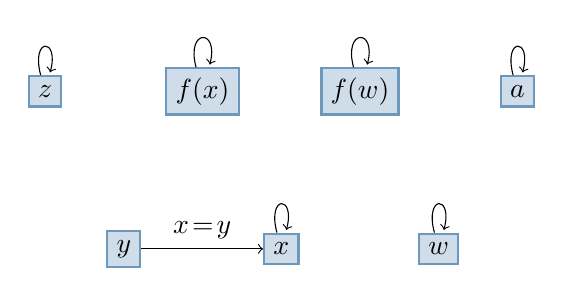
\begin{tikzpicture}[auto]

%
% Styles
%
\tikzstyle{vertex} = [rectangle,draw=oproverblue!60,fill=oproverblue!20,thick]

\node[vertex] (y) at  (  2, 0)  {$y$};
\node[vertex] (x) at  (  4, 0)  {$x$};
\node[vertex] (w) at  (  6, 0)  {$w$};
\node[vertex] (fx) at (  3, 2)  {$f(x)$};
\node[vertex] (fw) at (  5, 2)  {$f(w)$};
\node[vertex] (z) at  (  1, 2)  {$z$};
\node[vertex] (a) at  (  7, 2)  {$a$};

\draw[->] (y)  -- node {$x\!=\!y$} (x);
\path (x)  edge [loop above] (x);
\path (z)  edge [loop above] (z);
\path (w)  edge [loop above] (w);
\path (a)  edge [loop above] (a);
\path (fx) edge [loop above] (fx);
\path (fw) edge [loop above] (fw);

\end{tikzpicture}
}
    \only<3|handout:0>{\input{confl_2}}
    \only<4|handout:0>{\input{confl_3}}
    \only<5|handout:0>{\input{confl_4}}
    \only<6->{\input{confl_5}}
    \end{center}
  \end{overlayarea}
  \vfill
  \onslide<7->{
  On processing $a\not=z$, we call Explain( $a$, $z$ )
  }

\end{frame}

\begin{frame}[fragile]
  \frametitle{Lecture 7 - Exercize 2}
  
  \scriptsize

  We can store a reason of a Union inside the struct \verb|Node|

  \begin{verbatim}
  struct Node { 
    ...
    Node *  root;     // Points to class' representant
    Enode * reason;   // T-atom that caused union
  };
  \end{verbatim} 

  \begin{tabbing}
  aa \= a \= a \= a \= xxxxxxxxxxxxxxaaaaaaaaaaaaaaaaaaaaa \= asdasdasdasdasdasdasdasdasd \kill

     \> explanation $= \{\ \}$ \> \> \> \> // Global variable \\
   \\
   1 \> {\bf procedure} Explain( $s$, $t$ ) \\
   \\
   2 \> if ( $s == t$ ) return           \> \> \> \> // Nothing to explain \ldots \\
   \\
   3 \> while( $s.next \not= s$ )        \> \> \> \> // Collect reasons while moving to root \\
   4 \> \> if ( $s.reason == $ NULL )       \> \> \> // No reason: union caused by congruence \\
     \> \> \> // Let $s \equiv f( s_1, \ldots, s_n )$, $s.next \equiv f( t_1, \ldots, t_n )$ \\
   5 \> \> \> foreach $i \in \{ 1, \ldots, n \}$ \\
   6 \> \> \> \> Explain( $s_i$, $t_i$ ) \\
   7 \> \> else                             \> \> \> // Reason exists, save it \\
   8 \> \> \> explanation $=$ explanation $\cup\ \{ s.reason \}$ \\ 
   9 \> \> $s = s.next$ \\
   \\
   // Same ``while'' loop for $t$ \ldots

  \end{tabbing}

\end{frame}


\end{document}
